\documentclass[10pt, conference]{IEEEtran}
\hyphenation{op-tical net-works semi-conduc-tor}
\usepackage{graphicx}
\usepackage{fancyhdr}
\usepackage{url}
\usepackage{amsmath}
\usepackage{listings}
\usepackage{algorithm}
\usepackage{algorithmic}
\usepackage{lipsum}
\usepackage{bookmark}
\usepackage[normalem]{ulem}
\def\code#1{\texttt{#1}}
\useunder{\uline}{\ul}{}

\pagestyle{fancy}
\fancyhf{}
\lhead{\textsc{ELEN4020}}
\rhead{\textsc{Laboratory Exercise No 3}}
\rfoot{Page \thepage\ }


\begin{document}
\begin{titlepage}
\newcommand{\HRule}{\rule{\linewidth}{0.5mm}} % Defines a new command for the horizontal lines, change thickness here

\center % Center everything on the page
 
%----------------------------------------------------------------------------------------
%	HEADING SECTIONS
%----------------------------------------------------------------------------------------

\textsc{\LARGE University of Witwatersrand}\\[1.5cm] % Name of your university/college
%----------------------------------------------------------------------------------------
%	LOGO SECTION
%----------------------------------------------------------------------------------------


\includegraphics[scale=0.25]{Wits.png}% Include a department/university logo - this will require the graphicx package
 
 
%----------------------------------------------------------------------------------------
\textsc{\Large ELEN4020}\\[0.5cm] % Major heading such as course name
\textsc{\large Data Intensive Computing In Data Science}\\[0.5cm] % Minor heading such as course title



%----------------------------------------------------------------------------------------
%	TITLE SECTION
%----------------------------------------------------------------------------------------

\HRule \\[0.4cm]
{ \huge \bfseries Laboratory Exercise No 3}\\[0.4cm] % Title of your document
\HRule \\[1.5cm]
 
%----------------------------------------------------------------------------------------
%	AUTHOR SECTION
%----------------------------------------------------------------------------------------

\begin{minipage}{0.4\textwidth}
\begin{flushleft} \large
	\emph{Authors:}\\
	\textsc{Kishan Narotam - 717 931\\Jesal Chana - 603 177} 
\end{flushleft}
\end{minipage}
~
\begin{minipage}{0.4\textwidth}
\begin{flushright} \large
	\emph{Authors:} \\
	\textsc{Syed Hussain - 600 524\\Yusuf Ally - 604 973} 
\end{flushright}
\end{minipage}\\[2cm]

%----------------------------------------------------------------------------------------
%	DATE SECTION
%----------------------------------------------------------------------------------------

{\large 5\textsuperscript{th} April 2018}\\[2cm] % Date, change the \today to a set date if you want to be precise

%-------------------------------------------------------------------------------------

\vfill % Fill the rest of the page with whitespace

\end{titlepage}
%----------------------------------------------------------------------------------------


%----------------------------------------------------------------------------------------
%	MAIN BODY OF REPORT
%----------------------------------------------------------------------------------------

\section{Problem Description}
\label{Problem Description}
Two matrices, \emph{A} and \emph{B} of different dimensions and sizes must be multiplied together to produce the product matrix, \emph{C}, i.e. $C = A \times B$. In order for \emph{A} and \emph{B} to be multiplied, the rules of matrix multiplication must be met. These matrices are read in from text files, where the respective matrices are stored in the \emph{Matrix-Market} format. For example, if matrix \emph{A} is a $3\times4$ matrix, represented as:\\
\begin{center}
$A[3][4] = 
\begin{bmatrix}
a & b & c & d\\ 
e & f & g & h\\ 
i & j & k & l
\end{bmatrix}
$
\end{center}
This matrix will be read in from the file as follows:

\begin{center}
$
\begin{matrix}
3 & 4 & \\ 
0 & 0 & a\\ 
0 & 1 & b\\ 
2 & 3 & l\\ 
0 & 3 & d\\ 
1 & 0 & e\\ 
2 & 0 & i\\ 
1 & 1 & f\\ 
1 & 2 & g\\ 
2 & 1 & j\\ 
0 & 2 & c\\ 
2 & 2 & k\\ 
1 & 3 & h
\end{matrix}
$
\end{center}
The first line of the text file is the dimensions of the matrix, and following that, the first two elements of each line is the position, $A_{ij}$ of the third element in the line which is the value at that respective position within the matrix. The matrix could be an integer which is 4 bytes or a short floating point which too is 4 bytes. The elements of the matrix must be generated using the formula presented in equation~\ref{eqn1}:
\begin{equation}
\label{eqn1}
\begin{split}
A\langle i, j\rangle & = i *N_j + j
\end{split}
\end{equation}


\section{Background}
\label{Background}

\subsection{MapReduce}
\label{MapReduce}

\emph{MapReduce} is said to be the heart of the \emph{Apache Hadoop} software framework. This framework is written and built in order to process large amounts of data in parallel on large computer clusters, i.e. multiple nodes, with each node of the cluster having its own storage. There are two essential tasks that the program performs. The first of which is the \code{map} function which is said to take a set of data and convert it into another set. This \emph{mapper} filters and divides the work to the various nodes on the cluster (map). The individual elements are reduced to tuples, i.e. (\emph{key, value pairs})~\cite{WhatIs, IBM, Hadoop}.

The second task is the \code{reduce} function, which is responsible for taking the output from the \code{map}, which in turn becomes the input, and combines the data tuples into smaller set of tuples. The \emph{reducer} organizes and reduces the results from each node into a cohesive answer to a query. As the name suggests, the \code{reduce} function will always happen after the \code{map} function~\cite{WhatIs, IBM, Hadoop}.

An example of how the \emph{MapReduce} can be used could be as follows. Consider 5 files, containing two columns each. In terms of the framework, each file has a key and a value. Within each file, the first column is the name of a city and the second column would be the temperature on a random day. From these files, the goal is to find the maximum temperature for each city recorded. Using the \emph{MapReduce} framework, five mappers will work on its own file. The mapper will return the maximum temperature for each city. The reducer will then take the results from each mapper, and produce one output of each city and their maximum temperature recorded~\cite{IBM}.

\section{Algorithms}
\label{Algorithms}
Using the \emph{MrJob} framework, the algorithm was written in $Python$ programming language.

\subsection{Algorithm A: Using \emph{MapReduce} Repeated Times}
\label{Algorithm A}
Given two matrices, \emph{M} and \emph{N}, with the respective elements $m_{ij}$ and $n_{jk}$, the product, \emph{P}, will be $P=MN$, with the elements $p_{ik}$, where

\begin{center}
$p_{ik} = \sum_{j}^{} m_{ij}n_{jk}
$
\end{center}

The matrix will three key attributes, the first two would be regarded as the key, i.e. row number and column number, with the third being the value at that position. Matrix $M$ has the relation $M(I,J,V)$ with the corresponding tuples $(i,j,m_{ij})$. Matrix $N$ would have a similar relation as $N(J,K,W)$ with the tuples $(j,k,n_{jk})$. Since \emph{MapReduce} was created in order to handle larget sets of data, many large matrices are sparse, i.e. most elements are 0, and thus these tuples can be omitted. $i$, $j$ and $k$ could be implicit in the position of an element rather than written explicitly with the element itself. In a situation like this, the \code{map} function must be designed to construct $I$, $J$, and $K$ from the tuples from the position of the data~\cite{Book}.

The product output of the two matrices is a natural join, after the grouping, i.e. mapping. This means that between the two matrices, the $J$ attribute will be in common, resulting in the tuples $(i,j,k,v,w)$, where $(i,j,v)$ in $M$ and $j(j,k,w)$ in $N$. The natural join tuples, i.e. the five component tuple, represents a pair of matrix elements, $(m_{ij}, n_{jk})$. The desired tuple should have four components, $(i,j,k, v\times w)$ as this would represent the desired product result. Now that this relation has been established, one \code{map-reduce} operation can be done. The grouping can be done with $I$ and $K$ being the attributes for the grouping, the sum of $V \times W$ will be the aggregation~\cite{Book}.

Ultimately, the matrix multiplication can be cascaded of two \code{MapReduce} operations:

\begin{enumerate}
\item \textbf{\code{Map}}:
\begin{itemize}
	\item sends matrix element to key value pair:
		\subitem $m_{ij} \rightarrow (j, (M,i,m_{ij})$
		\subitem $n_{jk} \rightarrow (j, (N,k, n_{jk})$
\end{itemize}

\item \textbf{\code{Reduce}}:
\begin{itemize}
	\item for each key, $j$, examine list of associated values and produce the tuple $(i,j,m_{ij}n_{jk})$
	\item Output of this function is key $j$ with the list of all of the tuples of the from from $j$
\end{itemize}

\item \textbf{\code{Map}}:
\begin{itemize}
	\item this function is applied to the pairs which are the outputs from the prior \code{reduce} function\\
	\item The pairs are of the form $\rightarrow$ 
		\subitem $(j, [(i_1,k_1,v_1), (i_2,k_2,v_2),...,(i_q,k_q.v_q)])$
		\subitem $v_q = m_{i_qj} \times n_{jk_q}$
	\item From this, $p$ key-value pairs are produced:
		\subitem $((i_1,k_1),v_1),((i_2,k_2), v_2),...,((i_p,k_p),v_p)$

\end{itemize}
	
\item \textbf{\code{Reduce}}:
\begin{itemize}
	\item for each key, $(i,k)$, produce sum of list of values associated with the respective key
	\item The result $\rightarrow ((i,k),v)$ where $v$ is the value of the element in row $i$ and column $k$ in the product matrix $P$~\cite{Book}.

\end{itemize}
	
\end{enumerate}

\subsection{Algorithm B: Using One \emph{MapReduce} Step}
\label{Algorithm B}
A more efficient method of performing the basic matrix multiplication method would be to improve the two functions and ultimately use \code{MapReduce} only once to solve for $P=MN$. This is done by using the \code{map} function to create sets of elements that are needed to compute each element for the matrix $P$. One input element, will be turned into many key-value pairs, $(i,k)$ where $i$ is a row of $M$ and $k$ is a column of $N$~\cite{Book}.

\begin{enumerate}
\item \textbf{\code{Map}}:

\begin{itemize}
	\item for each element of $M$, $m_{ij}$, produce key-value pair:
		\subitem $((i,k), (M,j,m_{ij}))$ for $k = 1,2,....$ number of columns of $N$
	\item for each element of $N$, $n_{jk}$, produce key-value pair:
		\subitem $((i,k), (N,j,n_{jk}))$ for $i = 1,2,....$ number of rows of $M$
\end{itemize}


\item \textbf{\code{Reduce}}:
\begin{itemize}
	\item each key, $(i,k)$ will have a associated list with the values $(M,j,m_{ij})$ and $(N,j,n_{jk})$ for all possible values of $j$
	\item function must connect the two values on the list that have the same value of $j$ for each $j$

\end{itemize}
	
\end{enumerate}


\subsection{Algorithm C: Strassen Algorithm}
\label{Algorithm C}
The \emph{Strassen} Algorithm, or the \emph{Divide and Conquer} method for solving matrix multiplication can only be applied to square matrices, $n \times n$. However, the size of $n$ can only be in powers of 2. The multiplying matrices are divided into 4 smaller, sub matrices of size $\frac{n}{2}$~\cite{TutorialsPoint, GFG}. An example of the \emph{Strassen} algorithm would be as follows.

Given that $P=M\times N$, $M = \begin{bmatrix}
A &B \\ 
C &D 
\end{bmatrix}$, $N = \begin{bmatrix}
E &F \\ 
G &H 
\end{bmatrix}$ and $P = \begin{bmatrix}
I &J \\ 
K &L 
\end{bmatrix}$

Using \emph{Strassen}'s algorithm, the following equations must be calculated:
\begin{align*}
M_1&:= (A+C)\times (E +F)\\
M_2&:= (B+D) \times (G+H)\\
M_3&:=(A-D)\times (E+H)\\
M_4&:= A \times (F-H)\\
M_5&:= (C+D) \times (E)\\
M_6&:= (A+B) \times (H)\\
M_7&:= D \times (G-E)
\end{align*}
Then,
\begin{align*}
I&:=M_2+M_3-M_6-M_7\\
J&:=M_4+M_6\\
K&:=M_5 +M_7\\
L&:=M_1-M_3-M_4-M_5
\end{align*}

With regards to using the \code{MapReduce} functions, it could be implemented many ways, one of which would be using \emph{MapReduce} in a straight-forward fashion:
\begin{enumerate}
\item Compute $fv(A)$ and $fv(B)$ which takes $\log_n$ passes
\item Each value in $fv(A)$ is multiplied to the corresponding value from $fv(B)$\\

\emph{These two steps take one \code{MapReduce} pass}\\

\item Using various equations, the output from step 2 is transformed into the values in the product matrix.

\emph{This last step takes $\log_n$ \code{MapReduce} passes}~\cite{Conference}.
\end{enumerate}

\section{Function Description}
\label{Function Description}

\subsection{\code{MatrixGenerator}}
\label{MatrixGenerator}

Takes in an input (stored as N) from the user which defines the matrix dimensions (square matrix). A function is defined as create with parameter \code{matrix\_file}. \code{matrix\_file} is a text file with a unique name which will store a generated matrix.
A \code{for} loop is started, from $x = 0$ to $x = N$, which contains another \code{for} loop. This has an overall nested \code{for} loop structure and allows the program to create rows and coloumns of the same size. The second \code{for} loop, from $y = 0$ to $y = N$, generates a random integer from 1 to 10 using the \code{randint} function. This random integer is then written to the file, with a single space inbetween, using the file name provided via the parameter provided to the \code{create} function

The code then calls the function twice using the parameter file names \emph{File1ForLab3.txt} and \emph{File2ForLab3.txt}

\subsection{\code{MatrixMultiply1}}
\label{MatrixMultiply1}
The function aims to multiply two matrices together by first using a \emph{MapReduce} system to improve the speed and efficiency of the calculations when dealing with large data sets. The function reads in two text files which contain a matrix each. These matrices are in \emph{Matrix-Market} format and the first line defines their 2D parameters. The algorithm makes use of a single step \emph{MapReduce} before multiplication.\\

The \code{Map} function reads in the position (the $i$ and $j$ positions) and the corresponding value at that position. The matrix is then mapped, which means each value in the matrix is converted to a key-value format. The key being an identifier and the value is the corresponding element for that key. This is done by defining each element in terms of its co-ordinates and for Matrix 1 given each element a matrix identifier. The terms, in Matrix 1, are duplicated equal to the number of columns in Matrix 2 and are stored as the mapped results for Matrix 1. The format of these mapped views are show in equation~\ref{eqn2}.

\begin{equation}
\label{eqn2}
\begin{split}
Z_{ij} = ((i,k),(M,j, m_{ij})
\end{split}
\end{equation}
where:\\
$Z_{ij}$  = Final key-value pair for that particular value\\
$I$ = Co-ordinate of element in Matrix \\
$K$ = Iterator which goes from $1,2,…., N$ where $n$ = number of columns in matrix 2\\
$M$= Matrix identifier \\
$J$ = Second co-ordinate of the element within the matrix\\
$M_{i, j}$  = Value of element at the give $i-j$ position.\\

The result of the mapping is then passed to the \code{Reduc}e function which combines the relevant elements into a list. The elements that are combined need to have the same matrix identifier terms as well as the same value of $j$. These elements are then added to the key-value pair for that key and are joined to form a list of values. The same process is done for all possible matrix identifiers and $j$ values. The result from the Reduce Function is then multiplied and summed to give you a set of final key-value pairs which represents the product of matrix 1 and 2.


\subsection{\code{MatrixMultiply2}}
\label{MatrixMultiply2}
This method is similar to the standard \emph{MapReduce} method shown in Section~\ref{MatrixMultiply1}, however, it makes use of slightly different keys and two separate \emph{MapReduce} systems to improve on the speed of the first algorithm.\\

In the first round of Mapping the first matrix uses its $j$ values as the key rather than iterating to $k$ for each $i-j$ value as in Section~\ref{MatrixMultiply1}. For matrix 2 the $I$ value is used as the key instead. Example of this key value system is shown in equation~\ref{eqn3}.

\begin{equation}
\label{eqn3}
\begin{split}
Z_{ij} = (j,(M,i, m_{ij})
\end{split}
\end{equation}
where:\\
$Z_{ij}$  =  key-value pair\\
$J$ = $J$ position of element and key in this element ($I$ for matrix 2)\\
$M$ = Matrix identifier\\
$I$ = $I$ position of element\\
$M_{ij}$ = Element at position $i-j$\\

Once this mapping is done it is sent to the \code{Reduce} function which follows a similar pattern as in ection~\ref{MatrixMultiply1}, it appends the values of the same keys to form a list for that key and stores them. 
Once the initial \emph{MapReduce} is complete the second \emph{MapReduce} system a second \emph{MapReduce} is done where the matrix identifier and the the co-ordinate not used in the first mapping are used as the key and the list is appended with the values corresponding to those keys. 
The second \code{Reduce} function sums the values of those elements with the same key values.

\section{Pseudo Code}
\label{Pseudo Code}

\begin{algorithm}[h!]
\caption{The \code{Map} function~\cite{lendapp}}
\label{Map Algorithm}
\begin{algorithmic} 
\FOR {each element $m_{ij}$ of $M$}
	\STATE produce $(key,value)$ pairs $((i,k),(M,j,m_{ij}))$ for $k = 1,2,3...$ number of columns of $N$
\ENDFOR
\FOR {each element $n_{jk}$ of $N$}
	\STATE produce $(key,value)$ pairs $((i,k),(N,j,n_{jk}))$ for $i = 1,2,3...$ number of rows of $M$
\ENDFOR
\RETURN set of $(key,value)$ pairs that each key, $(i,k)$, has a list with values $(M,j,m_{ij})$ and $(N,j,n_{jk})$ for all possible values of $j$

\end{algorithmic}
\end{algorithm}

\begin{algorithm}[h!]
\caption{The \code{Reduce} function~\cite{lendapp}}
\label{Reduce Algorithm}
\begin{algorithmic} 
\FOR {each key $(i,k)$}
	\STATE sort values begin with $M$ by $j$ in $list_M$
	\STATE sort values begin with $N$ y $j$ in $list_N$
	\STATE multiply $M_{ij}$ and $n_{jk}$ for $j^{th}$ value of each list
	\STATE sum up $m_{ij} * n_{jk}$
\ENDFOR
\RETURN $(i,k)$, $\sum_{j=1}^{}m_{ij} * n_{jk}$


\end{algorithmic}
\end{algorithm}


\section{Final Code and Output}
\label{Final Code and Output}
The final code was developed in \emph{Python} using the \emph{MrJob} framework. The testing that was done calculated the time taken to multiply randomly generated matrices, using the \code{MatrixGenerator} function, using both matrix multiply functions created. These generated matrices are not sparse, i.e. have a density of $100\%$. An ASUS N550JV high performance laptop was used for testing. The machine has an \emph{Intel(R) Core(TM) i7-4700HQ CPU} with $12GB$ of RAM installed with a 64-bit operating system installed. The operating system installed is \emph{Windows 10 Pro} however for testing, a virtual machine was installed with the \emph{Ubuntu 16.04.3} 64-bit installed. $5GB$ of the total RAM is dedicated to the virtual machine. A custom created \emph{Makefile} was created in order to create the matrix using the \code{MatrixGenerator.py} file and to run the first and second algorithms, \code{MatrixMultiply1.py} and \code{MatrixMultiply2.py} respectively. The times taken to run each algorithm is written to respective text files.\\

Due to the limited resources, the maximum matrix size that was tested was $128 \times 128$ before any memory dumps occurred. Table~\ref{table} shows  the times recorded for each algorithm, and figure~\ref{graph} is the plotted results.

\begin{table}[h!]
\centering
\caption{Table showing the time taken, in seconds, to run each algorithm with matrices of various sizes}
\label{table}
\begin{tabular}{|c|c|c|}
\hline
{\ul \textbf{Matrix Size}} & {\ul \textbf{\code{MatrixMultiply1}}} & {\ul \textbf{\code{MatrixMultiply2}}} \\ \hline
\textbf{$2\times 2$} & 1.29130792618166 & 0.316252946853637 \\ \hline
\textbf{$4\times 4$} & 1.32429695129149 & 0.300330638885498 \\ \hline
\textbf{$8\times 8$} & 1.39224815369512 & 0.395497798919677 \\ \hline
\textbf{$16\times 16$} & 1.57556509972988 & 0.543861150741577 \\ \hline
\textbf{$32\times 32$} & 4.33468699455935 & 1.550762176513670 \\ \hline
\textbf{$64\times 64$} & 14.37436580669240 & 9.622877836227410 \\ \hline
\textbf{$128\times 128$} & 89.40903306018110 & 67.783106565475400 \\ \hline
\end{tabular}
\end{table}

\begin{figure}[h!]
\renewcommand{\thefigure}{\arabic{figure}}
\centering
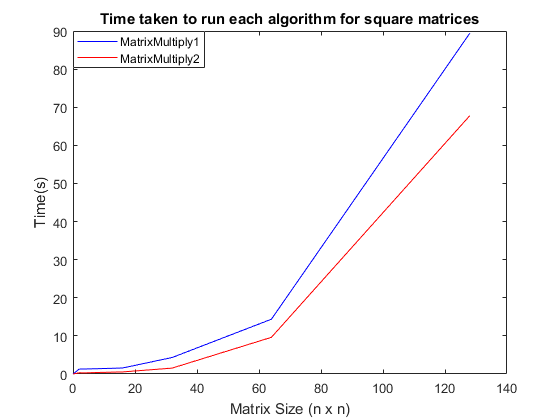
\includegraphics[scale=0.65]{Graph.png}
\caption{Graph showing time taken to run algorithm}
\label{graph}
\end{figure}

Although \code{MatrixMultiply1} should be more efficient, it seems that using the algorithm which utilizes the \code{MapReduce} function twice is more efficient. This could be due to the way the algorithm was executed, as \code{MatrixMultiply2} was executed using \emph{Python3} and \code{MatrixMultiply1} was executed using \emph{Python2}.


\section{Conclusion}
\label{Conclusion}
Matrix multiplication using \emph{MapReduce} framework was presented. A variety of algorithms and methods were presented using the \emph{MapReduce} framework in order to calculate matrix multiplication. It was shown that the algorithm that utilizes \code{MapReduce} twice was more efficient than the algorithm that uses it once.


\begin{thebibliography}{}

\bibitem{WhatIs}
Bigelow, SJ; Chu-Carroll, MC; \emph{What is MapReduce? - Definition from WhatIs.com}; \url{https://searchcloudcomputing.techtarget.com/definition/MapReduce}; Last Accessed: 04/04/2018

\bibitem{IBM}
IBM Analytics; \emph{What is MapReduce? | IBM Analytics}; \url{https://www.ibm.com/analytics/hadoop/MapReduce}; Last Accessed: 04/04/2018

\bibitem{Hadoop}
Hadoop; \emph{MapReduce Tutorial}; \url{https://hadoop.apache.org/docs/r1.2.1/mapred_tutorial.html}; Last Accessed: 04/04/2018

\bibitem{Book}
Leskovec, J; Rajaraman, A; Ullman, JD; \emph{Mining of Massive Datasets - Chapter 2}; Stanford University; Palo Alto, CA; March 2014

\bibitem{TutorialsPoint}
TutorialsPoint; \emph{Design and Analysis of Algorithms Strassen’s Matrix Multiplication}; \url{https://www.tutorialspoint.com/design_and_analysis_of_algorithms/design_and_analysis_of_algorithms_strassens_matrix_multiplication.htm}; Last Accessed: 04/04/2018

\bibitem{GFG}
GeeksforGeeks; \emph{Divide and Conquer | Set 5 (Strassen's Matrix Multiplication) - GeeksforGeeks}; \url{https://www.geeksforgeeks.org/strassens-matrix-multiplication/}; Last Accessed: 04/04/2018

\bibitem{Conference}
Deng, M; Ramanan, P; \emph{MapReduce Implementation of Strassen's Algorithm for Matrix Multiplication}; Proceedings of the 4th ACM SIGMOD Workshop on Algorithms and Systems fro MapReduce and Beyond Article No. 7; Chicago, IL, USA; 14-19 May 2017

\bibitem{lendapp}
Aytekin, M; \emph{Matrix Multiplication with MapReduce | lendapp}; \url{https://lendap.wordpress.com/2015/02/16/matrix-multiplication-with-mapreduce/}; Last Accessed: 04/04/2018

\end{thebibliography}




% that's all folks
\end{document}


